\documentclass[aspectratio=169,fontset=none]{ctexbeamer}
\usetheme{metropolis}
\usepackage{sourceserifpro,sourcesanspro,sourcecodepro}
\defaultCJKfontfeatures{Mapping=fullwidth-stop}
\IfFontExistsTF{Source Han Serif SC}{
  \setCJKmainfont{Source Han Serif SC}[
    UprightFont     = *-Regular,
    BoldFont        = *-Bold,
    ItalicFont      = 方正新楷体简体,
    BoldItalicFont  = *-Bold
  ]
  \setCJKsansfont{Source Han Sans SC}[
    UprightFont     = *-Regular,
    BoldFont        = *-Bold,
    BoldItalicFont  = *-Bold
  ]
  \setCJKmonofont{sarasa-mono-sc-regular.ttf}[
    ItalicFont      = sarasa-mono-sc-italic.ttf,
    BoldFont        = sarasa-mono-sc-bold.ttf,
  ]
}{
  \ctexset{fontset=fandol}
}

\AtBeginSubsection[]
{
\begin{frame}
\tableofcontents[currentsection,currentsubsection]
\end{frame}
}

\usepackage{minted}
\setminted{formatcom=\xeCJKVerbAddon}
\renewcommand{\emph}[1]{{\color{red}\bfseries #1}}
\newcommand{\pkg}[1]{\texttt{#1}}
\newcommand{\cls}[1]{\texttt{#1}}
\title{\pkg{amsthm} 宏包的使用 \& \LaTeX{} 代码的规范性 \& 内容与样式分离}
\author{死抠 \texttt{https://github.com/sikouhjw}}
\begin{document}
  \maketitle
  \begin{frame}{目录}
    \tableofcontents
  \end{frame}
  \begin{frame}[standout]{\LaTeX{} 工作室}
    \url{https://www.latexstudio.net/}
    
    
\includegraphics[height=0.7\textheight]{material/latex工作室.jpg}
  \end{frame}
  \begin{frame}[standout]{我的博客}
    \url{https://sikouhjw.gitee.io/}
  \end{frame}
  \section{\texorpdfstring{\pkg{amsthm}}{amsthm} 宏包的使用}
  \begin{frame}{\pkg{amsthm} 宏包中译本}
    GitHub 托管地址:\url{https://github.com/sikouhjw/amsthm-zh},基本都是机翻。
    \begin{center}
      \href{material/amsthdoc-zh-v1.0.pdf}{点我打开文档}
    \end{center}
  \end{frame}
  \subsection{\texorpdfstring{\pkg{amsthm}}{amsthm} 基础}
  \begin{frame}[fragile]{基本使用}
    加载 \pkg{amsthm} 宏包:
    \begin{minted}{latex}
\usepackage{amsthm}
    \end{minted}
    新定义一个定理类环境的方法:
    \begin{minted}{latex}
\newtheorem{环境名}{标题文本}
    \end{minted}
    例如:
    \begin{minted}{latex}
\newtheorem{lem}{Lemma}
    \end{minted}
    使用方法:
    \begin{minted}{latex}
\begin{lem} Text text ... \end{lem}
    \end{minted}
    输出:
    
\includegraphics{material/lem.pdf}
  \end{frame}
  \begin{frame}[fragile]{基本使用(续)}
    如果不想要编号,可以加 \mintinline{latex}{*} 号:
    \begin{minted}{latex}
\newtheorem*{lem}{Lemma}
    \end{minted}
    输出:
    
\includegraphics{material/lem2.pdf}
  \end{frame}
  \subsection{\texorpdfstring{\pkg{amsthm}}{amsthm} 进阶}
  \begin{frame}[fragile]{使用 \texttt{\textbackslash theoremstyle} 命令}
    我们可以发现,使用 \pkg{amsthm} 宏包直接 \mintinline{latex}{\newtheorem} 出来的定理类环境,有以下两个特点:
    \begin{itemize}
      \item 文本为斜体;
      \item 标题文本为粗体。
    \end{itemize}
    这是由于使用 \pkg{amsthm} 宏包时,如果没有指定定理类环境的风格,即没有使用 \mintinline{latex}{\theoremstyle} 命令,则使用的样式为 \texttt{plain}。
  \end{frame}

  \begin{frame}[fragile]{\pkg{amsthm} 宏包预定义的风格}
    \begin{itemize}
      \item \texttt{plain}:斜体文本,上面和下面额外的空间;
      \item \texttt{definition}:直立文字,在上面和下面留出额外的空间;
      \item \texttt{remark}:直立文字,上面或下面没有额外的空间.
    \end{itemize}
    下面的列表总结了通常与每种定理风格相关的结构类型.
    \begin{description}
      \item[plain] Theorem, Lemma, Corollary, Proposition, Conjecture, Criterion, Assertion
      \item[definition] Definition, Condition, Problem, Example, Exercise, Algorithm, Question, Axiom, Property, Assumption, Hypothesis
      \item[remark] Remark, Note, Notation, Claim, Summary, Acknowledgment, Case, Conclusion
    \end{description}
  \end{frame}

  \begin{frame}[fragile]{展示三种风格的效果}
    \begin{minipage}{\textwidth}
    \begin{minted}{latex}
\newtheorem{lem}{Lemma}
\theoremstyle{definition}
\newtheorem{defn}{Definition}
\theoremstyle{remark}
\newtheorem*{rem}{Remark}
    \end{minted}
    \end{minipage}
    \vskip 5pt
    \begin{minipage}[t]{0.6\textwidth}
    输入
    \begin{minted}{latex}
\begin{lem} 测试 test \end{lem}
\begin{defn} 测试 test \end{defn}
\begin{rem} 测试 test \end{rem}
    \end{minted}
    \end{minipage}%
    \begin{minipage}[t]{0.4\textwidth}
    输出
      \begin{figure}
        \centering
        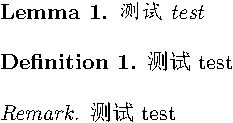
\includegraphics{material/三种定理风格.pdf}
      \end{figure}
    \end{minipage}
  \end{frame}

  \subsection{\texorpdfstring{\pkg{amsthm}}{amsthm} 高级应用}
  \begin{frame}[fragile]{使用 \texttt{\textbackslash newtheoremstyle} 命令}
    \begin{minted}{latex}
\newtheoremstyle{note}%   名字
  {3pt}{3pt}%             上面的空间、下面的空间
  {}%                     主体的字体
  {}%                     缩进量
  {\itshape}{:}%          定理头字体、定理头后标点符号
  {.5em}%                 定理头后的空间
  {}%                     定理头规范(可以为空,表示“正常”)
    \end{minted}
    \pause
    可以发现,\mintinline{latex}{\newtheoremstyle} 命令将定理类环境的样式大致分为这几个部分:
    \begin{itemize}
      \item 环境前、环境后的纵向距离;
      \item 主体、定理头的字体;
      \item 定理头的缩进。
    \end{itemize}
  \end{frame}

  \begin{frame}[fragile]{展示自定义风格的效果}
    设置环境前、环境后的纵向距离为 \mintinline{latex}{0pt},设置主体字体为 \mintinline{latex}{\kaishu},设置缩进为 \mintinline{latex}{2\ccwd},设置定理头的字体为 \mintinline{latex}{\bfseries}。
    \begin{minted}{latex}
\newtheoremstyle{mystyle}{0pt}{0pt}{\kaishu}{2\ccwd}%
{\bfseries}{.}{0pt}{}
    \end{minted}
    \begin{center}
      \href{material/高级效果.pdf}{点我查看效果}
    \end{center}
  \end{frame}

  \begin{frame}[fragile]{谁更好?}
    之前看的效果图的样式代码
    \begin{minted}{latex}
\newtheoremstyle{mystyle}{0pt}{0pt}{\kaishu}{2\ccwd}%
{\bfseries}{.}{0pt}{}
    \end{minted}
    与
    \begin{minted}{latex}
\vskip 0pt \begingroup
\indent\textbf{定理 1.}\kaishu 测试 test
\endgroup \vskip 0pt
    \end{minted}
    所达到的效果是一致的,但使用定理类环境——这种封装好的命令显然比手动修改样式更好——至于为什么好,我们先来讲讲 \LaTeX{} 代码的规范性。
  \end{frame}

  \section{\texorpdfstring{\LaTeX{}}{LaTeX} 代码的规范性}
  \begin{frame}
    想知道什么叫规范之前,必须先知道什么叫\emph{不规范},事实上不规范的代码在网络上是非常常见的,我这里给一段槽点无处不在的数学建模论文代码。
  \end{frame}

  \begin{frame}[fragile]{导言区}
    \begin{minipage}[t]{0.5\textwidth}
      \begin{minted}{latex}
\documentclass{article}
\usepackage{ctex}
\usepackage{indentfirst}
\setlength{\parindent}{2em}
\usepackage{fancyhdr}
\usepackage{lastpage}
\usepackage{array}
\usepackage{color}
\usepackage{hyperref}
\usepackage{xcolor}
\usepackage{color}
      \end{minted}
    \end{minipage}%
    \begin{minipage}[t]{0.5\textwidth}
      槽点大致有如下几点:
      \begin{itemize}
        \item \begin{minted}{latex}
\usepackage{indentfirst}
\setlength{\parindent}{2em}
        \end{minted}
        \pkg{ctex} 宏包已经设置了首段缩进,为什么要写两句\emph{没用}的废代码呢?
        \item \pkg{hyperref} 宏包一般是最后几个加载的,这算是常识了;
        \item \pkg{color} 与 \pkg{xcolor} 重复加载;
      \end{itemize}
    \end{minipage}
  \end{frame}

  \begin{frame}[fragile]
    \begin{minipage}[t]{0.45\textwidth}
      \begin{minted}{latex}
\usepackage{ulem}
\usepackage{CJKfntef}
\usepackage{ulem}
\usepackage{listings}
\lstset{language=Matlab}
\usepackage{lipsum}
\usepackage{minted}
\usepackage{lipsum}
\renewcommand%
{\contentsname}%
{\centerline{目录}}
      \end{minted}
    \end{minipage}%
    \begin{minipage}[t]{0.55\textwidth}
      \begin{itemize}
        \item \pkg{CJKfntef} 是用于产生下划线等效果的宏包,是属于 \pkg{cjk} 时代的宏包,\pkg{ulem} 也是用于产生下划线的宏包,那么为什么要重复加载呢?\pkg{ulem} 还加载了两次;
        
        目前推荐的用于产生下划线的宏包是 \pkg{xeCJKfntef},是 \pkg{xeCJK} 的子包,需要手动加载;
        \item \pkg{lipsum} 加载两次;
        \item \pkg{minted} 是用于排版代码的宏包,可明明已经加载了 \pkg{listings} 宏包;
        \item \mintinline{latex}{\contentsname} 已经被 \pkg{ctex} 宏包汉化为\emph{目录}了,废代码;
      \end{itemize}
    \end{minipage}
  \end{frame}

  \begin{frame}[fragile]{正文}
    \begin{minipage}[t]{0.5\textwidth}
      \begin{minted}{latex}
\begin{spacing}{1.5}
  文字文字文字
\end{spacing}
\begin{spacing}{1.5}
  文字文字文字
\end{spacing}
\section*{一、问题的提出}
\subsection*{1.1~~~~问题背景}
\subsection*{1.2~~~~问题咋来的}
\section*{二、问题的分析}
\subsection*{2.1~~~~问题一的分析}
\caption*{图4.3~~~~问题一的结果图}
      \end{minted}
    \end{minipage}%
    \begin{minipage}[t]{0.5\textwidth}
      \begin{itemize}
        \item \mintinline{latex}{spacing} 环境是用来调整行间距的,这么做太麻烦了,不如使用 \mintinline{latex}{\linespread} 一劳永逸;
        \item 手写所有章节、图表编号,我也不知道该怎么说,可能跟习惯使用 word 有关。
      \end{itemize}
    \end{minipage}
  \end{frame}

  \begin{frame}{什么是规范?}
    虽然我们没办法对规范性下定义,但我们可以指出不规范的 \LaTeX{} 代码的几个特点:
    \begin{itemize}
      \item 手写编号;
      \item 手动调节样式;
      \item 重复加载宏包、不知作用就胡乱加载宏包;
      \item 做重复的、无用的工作。
    \end{itemize}
    代码不规范可能带来的几个坏处:
    \begin{itemize}
      \item 宏包冲突(参考《\href{https://wenda.latexstudio.net/q-2478.html}{使用newtxtext、直立积分号newtxmath包出现与textcomp宏包选项冲突}》);
      \item 老板的一句话让你又要花几个小时去修改样式(比如把定理类环境的 \mintinline{latex}{\bfseries} 换为红色,比如将 \mintinline{latex}{\subsection} 的样式改为 \S 1.1);
      \item 你队友增加 / 减少一个章节 / 图表,你需要修改后续所有的数字。
    \end{itemize}
  \end{frame}

  \begin{frame}{思考}
    如果我们想避免这种重复劳动(修改样式),我们应该怎么做?结合前面学习的 \pkg{amsthm} 宏包,我们复习一下 \pkg{amsthm} 宏包将定理类环境分为哪几个部分:\pause
    \begin{itemize}
      \item 环境前、环境后的纵向距离;
      \item 主体、定理头的字体;
      \item 定理头的缩进;
      \item 定理头后的标点符号;
      \item 标点符号后与正文的横向距离。
    \end{itemize}
    \pause
    这种将一个环境分为若干个部分,分别设定其样式的思想就叫做\emph{内容与样式分离}。
  \end{frame}

  \section{什么是内容与样式分离?}
  \begin{frame}[fragile]{什么是内容与样式分离?}
    \emph{内容与样式分离}:一篇文档的\emph{实际内容}和\emph{逻辑结构}与这篇文档呈现给读者看到的\emph{样式}是相互独立的。\pause

    举个例子,如果数学建模论文一级标题要求:
    \begin{itemize}
      \item 居中;
      \item 黑体、三号字体;
      \item number 为 \mintinline{latex}{\chinese} 格式;
      \item number 后面接顿号。
    \end{itemize}
    表现为
    \begin{center}
      \zihao{3}一、问题的提出
    \end{center}
  \end{frame}
  \begin{frame}[fragile]
    在 Word 中,很多人可能会
    \begin{enumerate}
      \item 输入文字:「一、问题的提出」;
      \item 选中文字,居中、设置字体为黑体、设置字号为三号。
    \end{enumerate}
    等价于 \LaTeX{} 中的
    \begin{minted}{latex}
\begin{center}
  \zihao{3}\heiti 一、问题的提出
\end{center}
    \end{minted}
    \pause
    结合之前所学,我们知道,这么做是十分不推荐的,因为
    \begin{itemize}
      \item 手写编号;
      \item 手写样式。
    \end{itemize}
    \pause
    \LaTeX{} 提供了预定义的章节命令,只需要修改它的样式即可,而不是\emph{手写样式}。我们来看看 \mintinline{latex}{\section} 的定义,继续加深对\emph{内容与样式分离}的理解。
  \end{frame}
  \begin{frame}[fragile]{\texttt{\textbackslash section} 命令}
    \mintinline{latex}{\section} 在 \cls{article} 文档类里面的定义可以通过命令行执行
    \begin{minted}{latex}
latexdef -c {article} -s \section
    \end{minted}
    找到,结果为
    \begin{minted}{latex}
% article.cls, line 302:
\newcommand\section{\@startsection%
  {section}{1}{\z@}%
  {-3.5ex \@plus -1ex \@minus -.2ex}%
  {2.3ex \@plus.2ex}%
  {\normalfont\Large\bfseries}}
    \end{minted}
  \end{frame}
  \begin{frame}[fragile]
    \begin{minted}{latex}
% article.cls, line 302:
\newcommand\section{\@startsection%
  {section}{1}{\z@}%
  {-3.5ex \@plus -1ex \@minus -.2ex}%
  {2.3ex \@plus.2ex}%
  {\normalfont\Large\bfseries}}
    \end{minted}
    可以发现,\mintinline{latex}{\section} 命令在格式上无非是干了这几件事
    \begin{itemize}
      \item 缩进 \mintinline{latex}{\z@} 距离;
      \item 设置前后纵向间距;
      \item 设置字体大小为 \mintinline{latex}{\Large}、粗细为 \mintinline{latex}{\bfseries}。
    \end{itemize}
  \end{frame}
  % \begin{frame}[fragile]{IF……}
  %   我们没有必要也不应该抛弃这种封装好的格式,而去\emph{手写样式}。

  %   那么如果你在写一本书,书中有上百个章节格式,如果你是\emph{手写样式},你需要反复的 copy,如果你的老板 / 编辑告诉你:「这里要这么改……」,那么你是否要手动改上百处?
  % \end{frame}

  \begin{frame}
    看到现在,你应该对\emph{内容与样式分离}有了初步的认识,但这还不够,这种思想充斥在 \LaTeX{} 的各个角落里。我们先来看一下用 \LaTeX{} 写一本书的代码结构是怎样的。
  \end{frame}

  \begin{frame}[fragile]{一本书的代码结构}
    \begin{minipage}[t]{0.5\textwidth}
    \begin{minted}{latex}
\documentclass{book}
\usepackage{makeidx}
\makeindex
\bibliographystyle{plain}
\begin{document}
\frontmatter
\maketitle
\include{preface}
\tableofcontents
\mainmatter
\include{chapter1}
    \end{minted}
    \end{minipage}%
    \begin{minipage}[t]{0.5\textwidth}%
      \begin{minted}{latex}
\include{chapter2}
...
\appendix
\include{appendixA}
...
\backmatter
\include{prologue}
\bibliography{books}
\printindex
\end{document}
      \end{minted}
    \end{minipage}
    \pause\vskip 2.5pt
    我们抽出其中的一部分,看看常见的 \mintinline{latex}{\frontmatter} 是怎么定义的。
  \end{frame}

  \begin{frame}[fragile]
    命令行输入
    \begin{minted}{latex}
latexdef -c {book} -s \frontmatter
    \end{minted}
    得到
    \begin{minted}{latex}
% book.cls, line 284:
\newcommand\frontmatter{%
    \cleardoublepage\@mainmatterfalse
  \pagenumbering{roman}}
    \end{minted}
    可以看出,\mintinline{latex}{\frontmatter} 大概做了两件事:
    \begin{itemize}
      \item 换页;
      \item 设置页码样式为 \mintinline{latex}{\roman}。
    \end{itemize}
    \pause
    那么是否可以用 \mintinline{latex}{\pagenumbering{roman}} 代替 \mintinline{latex}{\frontmatter} 呢?\pause 答案是不能的,因为 \mintinline{latex}{\frontmatter} 命令主要的功能不是设置页码样式,而是代表\emph{开始前言}。
  \end{frame}
  \begin{frame}[fragile]
    我们在写书的时候,需要区分的是\emph{前言}、\emph{正文}、\emph{附录}和\emph{后记},而不是页码样式为 \mintinline{latex}{\roman} 和页码样式为 \mintinline{latex}{\arabic},你完全可以将页码样式定义成你喜欢的样式,比如 \mintinline{latex}{\alph},比如 \mintinline{latex}{\S\thepage},页码样式只是为了区分不同的文档结构才设置的不同。
  \end{frame}
    
  \begin{frame}[standout]{我理解的内容与样式分离}
    注重命令的意义,将想排版的内容分割、赋予其不同的意义,从而保留样式的可变性、自由度,我认为这才是\\[8pt]
    {\huge\emph{内容与样式分离}}\\[5pt]
    的内涵所在。
  \end{frame}

  \begin{frame}{关于}
    \vspace*{1.2cm}
    本幻灯片:\url{https://github.com/sikouhjw/LaTeX-live}

    许可证:LaTeX Project Public License v1.3c
    \vspace{2.8cm}
    \begin{flushleft}
      \tiny
      Beamer 主题:Metropolis\\
      正文字体:Source Han Sans SC + Source Sans Pro\\
      等宽字体:Sarasa Mono SC + Source Code Pro
    \end{flushleft}
  \end{frame}

  \begin{frame}[standout]
    \huge \textbf{\texttt{\textbackslash bye}}
  \end{frame}
\end{document}